\documentclass[10pt]{article}
\usepackage[letterpaper,margin=1in]{geometry}
\usepackage{times}
\usepackage[T1]{fontenc}
\usepackage{amsmath,amssymb,amsthm}
\usepackage{graphicx}
\usepackage{booktabs}
\usepackage[numbers,sort&compress]{natbib}
\usepackage{microtype}
\usepackage{xcolor}
\usepackage[hidelinks]{hyperref}
\usepackage{caption}
\captionsetup{font=small}
\setlength{\bibsep}{1pt}

\newtheorem{theorem}{Theorem}
\newcommand{\C}{\mathcal{C}}
\newcommand{\cond}{\mathrm{cond}}
% auto-generated by scripts/make_paper_macros.py
\newcommand{\DubAbstract}{the verifier proves the barrier conditions on 99.4\% of the domain volume and certifies $X_0\subseteq\C$, yet returns 524 validated counterexamples that uniform sampling hits at a rate of only $\sim\!10^{-5}$ -- exactly the failure mode that motivates formal verification.}
\newcommand{\DubResults}{After 40 CGIS rounds a re-verification that processes 1{,}073{,}497 boxes proves P1--P2 on 99.4\% of $\mathrm{vol}(D)$ (381{,}104 leaves, 2{,}949 closed by Z3) and P0 on all of $X_0$ (22{,}399 leaves), but stops after collecting 524 validated counterexamples, so the status is \textsc{falsified} and no certificate is issued. All violations sit on the edge of $\C$ close to the obstacle at near-zero speed, where $\dot B$ can only be changed through $\partial B/\partial v$ and $\partial B/\partial\theta$. The learned policy is conservative: at $v=0.6$ the set $\C$ is small (Fig.~\ref{fig:main}) and the controller mostly brakes to rest. This failure is nearly invisible empirically: 2{,}000{,}000 uniform samples contain only 23 violating states, and 100 rollouts from $X_0$ and $\C$ (10\,s) never leave $\C$. Rollouts started at verifier counterexamples, however, leave $\C$ in 41/50 cases (none reaches the obstacle), confirming that the violations are real invariance failures.}
\newcommand{\DubFigure}{figures/dubins_slices.pdf}
\newcommand{\DubFigCaption}{Dubins car: slices $(p_x,p_y)$ of $\C$ at headings $\theta\in\{0,\pi/2,\pi,-\pi/2\}$ for $v=0$ (top) and $v=0.6$ (bottom); obstacle in red.}


\title{\textbf{CertiControl-NN: Sound Branch-and-Bound Certificates for\\Neural Control Barrier Functions with SMT-Guided Synthesis}}
\author{Anonymous authors\\{\small Workshop submission}}
\date{}

\begin{document}
\maketitle
\vspace{-2em}
\begin{abstract}
\noindent
Neural controllers trained by reinforcement or imitation learning are evaluated by simulation, which cannot rule out failures in unvisited regions of a continuous state space. We present \emph{CertiControl-NN}, an open-source, laptop-scale framework that co-trains a neural controller $\pi_\theta$ with a neural control barrier function (NCBF) $B_\phi$ and \emph{proves} forward invariance of $\{B_\phi\ge 0\}$ for all states of a continuous domain. The closed-loop certificate $[B,\ \nabla B\cdot(f+g\pi)+\gamma B]$ is written once as a forward-mode computational graph and executed by three backends: tensors (training), sound interval arithmetic and CROWN linear relaxation via \texttt{auto\_LiRPA} (bounding), and Z3 (pointwise decision over CROWN's linear bounds and an exact unsafe set). A branch-and-bound verifier discharges four properties---invariance, unsafe-set avoidance, domain containment and non-triviality---and returns validated counterexamples that drive counterexample-guided inductive synthesis (CGIS). An independent checker re-proves each stored proof leaf. On a torque-limited inverted pendulum the loop certifies in 3 rounds; CROWN shrinks the proof $1500\times$ relative to interval bounds and Z3 closes boundary-straddling boxes. On a 4-D Dubins car with an obstacle and walls, \DubAbstract
\end{abstract}

\section{Introduction}
Control barrier functions (CBFs) certify safety through forward invariance of a super-level set~\cite{ames2019cbf,prajna2004barrier}. Learning CBFs with neural networks makes them expressive enough for nonlinear, input-constrained systems~\cite{dawson2023survey,zhao2020synthesizing}, but a learned certificate is only as good as its verification: a network that satisfies the CBF inequality on millions of samples may still violate it on a set of positive measure. Existing pipelines verify neural certificates with $\delta$-complete SMT solvers~\cite{chang2019neural,abate2021fossil} (sound but slow beyond small networks) or with linear-relaxation bound propagation~\cite{wang2023simultaneous} (fast, but inconclusive boxes must be refined).

We combine both in a CGIS loop~\cite{solarlezama2006sketching}. Our contributions are: (i) a \emph{single-source} closed-loop certificate graph with an exact forward-mode Lie derivative that is simultaneously trainable, IBP/CROWN-boundable~\cite{gowal2018ibp,zhang2018crown,xu2020autolirpa} and Z3-encodable~\cite{demoura2008z3}; (ii) a Z3 step that reasons \emph{pointwise} about the disjunction ``outside $\C$ or CBF condition holds'' over CROWN's linear bounds with the unsafe set encoded exactly, closing boxes that straddle $\partial\C$; (iii) a non-triviality property that rules out the vacuous certificate, a smooth-band training loss that lets the optimizer shrink $\C$, and an independent proof checker; (iv) an end-to-end open-source implementation running on an 8\,GB laptop CPU.

\section{Problem Formulation}
Consider $\dot x=f(x)+g(x)u$, $x\in\mathbb R^n$, with actuator box $u\in[u_{\min},u_{\max}]$, a hyper-rectangular domain $D$ (some coordinates may be periodic), unsafe set $X_u=\bigcup_i\{h_i(x)\le 0\}$ and initial set $X_0$. The controller $\pi_\theta(x)=u_{\rm mid}+u_{\rm half}\tanh(\mathrm{MLP}_\theta(\psi(x)))$ satisfies the input limits by construction; $B_\phi(x)=\mathrm{MLP}_\phi(\psi(x))$ uses tanh activations and a feature map $\psi$ (e.g.\ $(\cos\theta,\sin\theta)$ for headings). Let $\cond(x)=\nabla B(x)\cdot(f(x)+g(x)\pi(x))+\gamma B(x)$ and $\C=\{x\in D:B(x)\ge 0\}$. We certify
\begin{align*}
&\textbf{P1: } \forall x\in D:\ B(x)\ge 0\Rightarrow \cond(x)\ge 0, &&\textbf{P2: } \forall x\in D\cap X_u:\ B(x)<0,\\
&\textbf{P3: } \forall x\in\partial D \text{ (non-periodic faces)}:\ B(x)<0, &&\textbf{P0: } \forall x\in X_0:\ B(x)>0.
\end{align*}
\begin{theorem}
Under P0--P3, every closed-loop trajectory with $x(0)\in \C$ (in particular $x(0)\in X_0$) satisfies $x(t)\in\C\subset D\setminus X_u$ for all $t\ge 0$.
\end{theorem}
\noindent\emph{Sketch.} By P3, $\C$ is compact and contained in the interior of $D$, so a trajectory can only leave $\C$ through $\{B=0\}$; on $\C$, P1 gives $\dot B\ge-\gamma B$, and the comparison lemma yields $B(x(t))\ge e^{-\gamma t}B(x(0))\ge 0$. P2 gives $\C\cap X_u=\emptyset$ and P0 gives $X_0\subseteq\C$. Since $\gamma' B\ge\gamma B$ on $\C$, a certificate for $\gamma$ also holds for all $\gamma'\ge\gamma$. \hfill$\square$

\section{Method}
\textbf{Verifiable Lie derivative.} Rather than differentiating through autograd twice, we propagate a tangent through the network: $z=Wh+b,\ dz=W\,dh,\ h'=\tanh z,\ dh'=\tanh'(z)\odot dz$, seeded with $d\psi=J_\psi(x)\,(f+g\pi)$. The certificate $x\mapsto[B,\cond]$ is thus a plain feed-forward graph of linear, $\tanh$, $\sin$, $\cos$ and product nodes. A backend-dispatch layer runs the \emph{same} code on tensors, on intervals and on Z3 affine forms.

\textbf{Sound bounding.} Our interval backend works in float64 with outward widening dominating each operation's rounding error, exact extremum detection for $\sin/\cos$ and a unimodal enclosure of $\tanh'$. CROWN bounds and linear bounding functions $\underline A x+\underline b\le[B,\cond](x)\le\overline Ax+\overline b$ are obtained from \texttt{auto\_LiRPA}~\cite{xu2020autolirpa} in float64; we intersect IBP and CROWN bounds. A box of $D$ is discharged if $\overline B<-\tau$ (outside $\C$) or if $\underline{\cond}\ge\tau$ and it provably misses $X_u$; face boxes need $\overline B<-\tau$; $X_0$ boxes need $\underline B>\tau$ or to provably miss $X_0$ ($\tau=10^{-8}$).

\textbf{Z3 step.} For an undischarged box $R$, Z3 decides
$\exists x\in R:\ \overline A_Bx+\overline b_B\ge-\tau\ \wedge\ (\underline A_c x+\underline b_c<\tau\ \vee\ \textstyle\bigvee_i h_i(x)\le 0)$
over exact rationals, with $h_i$ encoded exactly (e.g.\ the obstacle disc is a polynomial constraint). UNSAT proves the box \emph{pointwise}, which is strictly stronger than the box-level test: the linear lower bound of $\cond$ may be negative only where the linear upper bound of $B$ is already negative. A SAT model is evaluated on the real network and becomes a counterexample only if it violates a property; otherwise the box is split. We also provide a full-graph QF\_LRA encoding (mean-value enclosures for smooth scalar functions, McCormick envelopes~\cite{mccormick1976} for products, dyadic coefficient rounding with sound loosening); it is exact up to relaxation but practical only for small networks.

\textbf{Branch and bound.} Boxes are processed breadth-first in batches: concrete falsification at two points, IBP, CROWN, Z3 (for boxes below a size threshold), bisection of the widest (domain-normalised) coordinate. Falsified large boxes are still split to explore their remainder. Leaves and their proving method are stored.

\textbf{CGIS training.} The loss is $\mathcal L=w_1\mathcal L_{\rm lie}+w_2\mathcal L_{\rm unsafe}+w_3\mathcal L_{\partial D}+w_0\mathcal L_{X_0}+w_c\mathcal L_{\rm CGIS}+w_\ell\mathcal L_{\rm Lip}$ with hinge terms of margin $m$ and $\mathcal L_{\rm CGIS}=\max(0,m-\cond(x_{\rm cex}))$ on validated counterexamples and jittered copies. The Lie term is weighted by $\sigma((B+\delta)/\tau)$ rather than a hard mask: its gradient with respect to $B$ lets the optimiser \emph{exclude} states where the condition is infeasible, which we found necessary to avoid thin, unverifiable ``arms'' of $\C$. Half of each batch is drawn from the band $B\ge-\delta$, and a finite-difference Lipschitz penalty on $\pi$ prevents bang-bang controllers whose relaxations are loose.

\textbf{Proof checking.} From stored weights, the checker verifies that leaves lie in their region and that their volumes sum to its volume (leaves of a bisection tree are interior-disjoint), then re-proves every leaf with its recorded method.

\section{Experiments}
All runs use two CPU threads (float64). Networks have two hidden tanh layers of width 32; $\gamma=1$.

\begin{figure}[t]
\centering
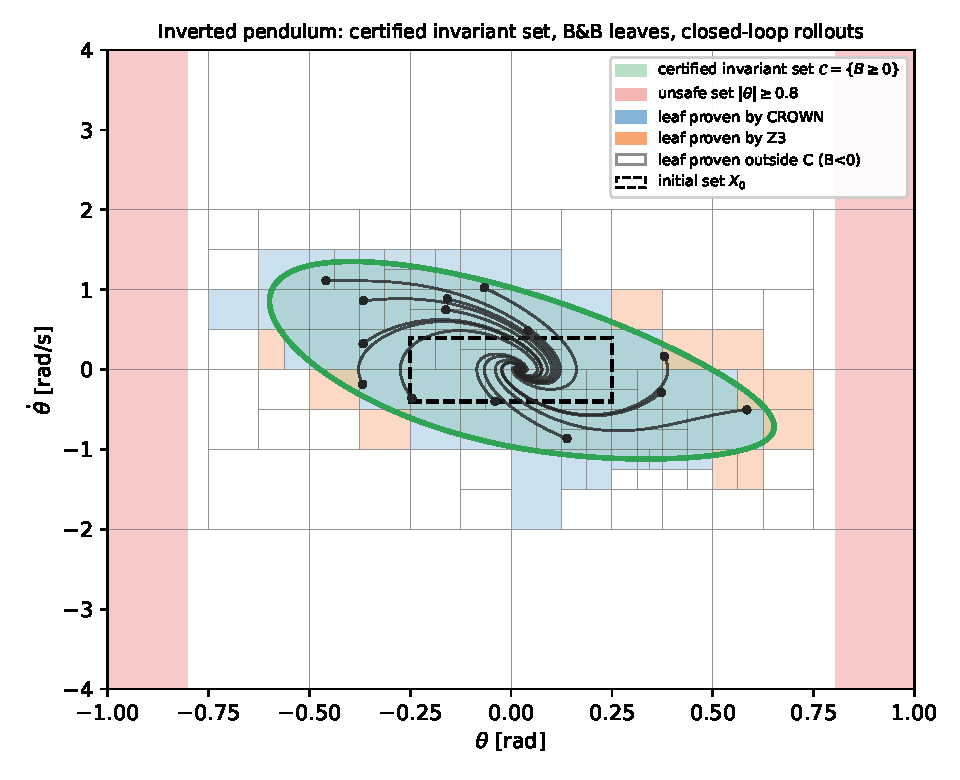
\includegraphics[width=0.49\linewidth]{figures/pendulum_certified.pdf}\hfill
\includegraphics[width=0.49\linewidth]{\DubFigure}
\caption{Left: pendulum ($\theta,\dot\theta$); certified invariant set (green), unsafe set $|\theta|\ge 0.8$ (red), proof leaves by method, and closed-loop rollouts. Right: \DubFigCaption}
\label{fig:main}
\vspace{-1em}
\end{figure}

\textbf{Inverted pendulum.} $\ddot\theta=(g/l)\sin\theta-b\dot\theta+u$, $|u|\le 6$, $D=[-1,1]\times[-4,4]$, $X_u=\{|\theta|\ge0.8\}$, $X_0=[-0.25,0.25]\times[-0.4,0.4]$. Since $u_{\max}<g\sin 0.8$, the torque limit rather than $X_u$ bounds the viable set. CGIS certified the system in 3 rounds (72 and 7 counterexamples in rounds 0--1). The final proof has 140 domain leaves (129 CROWN, 11 Z3), 7 face leaves and 1 $X_0$ leaf; verification takes 2.7\,s and the checker accepts it in 1.5\,s (Fig.~\ref{fig:main}). The proof also holds for $\gamma\in\{0.25,\dots,4\}$.

\begin{table}[h]
\centering\small
\begin{tabular}{lcccc}
\toprule
bounding method (final pendulum networks) & status & boxes processed & proof leaves & time [s]\\
\midrule
IBP only & certified & 433\,573 & 216\,787 & 2.5\\
IBP + CROWN (\texttt{auto\_LiRPA}) & certified & 329 & 165 & 2.5\\
IBP + CROWN + Z3 (ours) & certified & 279 & 140 (11 Z3) & 2.5\\
\bottomrule
\end{tabular}
\caption{Verifier ablation. CROWN reduces the proof size by three orders of magnitude; the pointwise Z3 step removes a further 15\% of leaves by closing boxes that straddle $\partial\C$.}
\label{tab:abl}
\vspace{-1em}
\end{table}

\textbf{Dubins car.} $\dot p_x=v\cos\theta,\ \dot p_y=v\sin\theta,\ \dot\theta=u_1,\ \dot v=u_2$, $|u_1|,|u_2|\le 2$, $D=[-2,2]^2\times S^1\times[-1,1]$ (walls and speed limits are faces of $D$), obstacle $\|p\|\le 0.6$, $X_0$: $|p_x|,|p_y|\le1.4$, $|v|\le0.25$, clearance $\ge0.35$. A soft imitation term towards a goal-seeking nominal controller keeps $\pi$ useful. \DubResults

\textbf{Empirical cross-checks.} Independent of the proofs, 2\,M uniform samples show no violation of P0--P3 for the certified pendulum, and 100 scipy RK45 rollouts (10\,s) started in $X_0$ or $\C$ never leave $\C$.

\section{Limitations and Conclusion}
CROWN is computed in float64 without directed rounding; we absorb rounding with a $10^{-8}$ margin, as is common practice, whereas IBP and Z3 are sound in real arithmetic. Guarantees concern the continuous-time model and the stored weights, not sampling, delays or model error. Input-space branch-and-bound grows exponentially with state dimension: 2-D problems verify in seconds, 4-D ones require millions of boxes. The Dubins experiment shows the other side of the coin: the verifier refuses to certify a controller that looks perfect in simulation, and CGIS did not remove the last violations within 40 rounds. Promising directions are optimised relaxations ($\alpha,\beta$-CROWN), verification-aware training, and learned branching. CertiControl-NN shows that sound, independently checkable safety certificates for neural controllers are attainable with open-source tools on a laptop.

{\small
\bibliographystyle{plainnat}
\begin{thebibliography}{99}
\bibitem[Ames et al.(2019)]{ames2019cbf} A.~D. Ames, S.~Coogan, M.~Egerstedt, G.~Notomista, K.~Sreenath, and P.~Tabuada. Control barrier functions: Theory and applications. In \emph{European Control Conference (ECC)}, 2019.
\bibitem[Prajna and Jadbabaie(2004)]{prajna2004barrier} S.~Prajna and A.~Jadbabaie. Safety verification of hybrid systems using barrier certificates. In \emph{HSCC}, 2004.
\bibitem[Dawson et al.(2023)]{dawson2023survey} C.~Dawson, S.~Gao, and C.~Fan. Safe control with learned certificates: A survey of neural Lyapunov, barrier, and contraction methods for robotics and control. \emph{IEEE Transactions on Robotics}, 2023.
\bibitem[Zhao et al.(2020)]{zhao2020synthesizing} H.~Zhao, X.~Zeng, T.~Chen, and Z.~Liu. Synthesizing barrier certificates using neural networks. In \emph{HSCC}, 2020.
\bibitem[Chang et al.(2019)]{chang2019neural} Y.-C. Chang, N.~Roohi, and S.~Gao. Neural Lyapunov control. In \emph{NeurIPS}, 2019.
\bibitem[Abate et al.(2021)]{abate2021fossil} A.~Abate, D.~Ahmed, A.~Edwards, M.~Giacobbe, and A.~Peruffo. FOSSIL: A software tool for the formal synthesis of Lyapunov functions and barrier certificates using neural networks. In \emph{HSCC}, 2021.
\bibitem[Wang et al.(2023)]{wang2023simultaneous} X.~Wang, L.~Knoedler, F.~B. Mathiesen, and J.~Alonso-Mora. Simultaneous synthesis and verification of neural control barrier functions through branch-and-bound verification. \emph{arXiv:2311.10438}, 2023.
\bibitem[Solar-Lezama et al.(2006)]{solarlezama2006sketching} A.~Solar-Lezama, L.~Tancau, R.~Bod\'ik, S.~Seshia, and V.~Saraswat. Combinatorial sketching for finite programs. In \emph{ASPLOS}, 2006.
\bibitem[Gowal et al.(2018)]{gowal2018ibp} S.~Gowal, K.~Dvijotham, R.~Stanforth, R.~Bunel, C.~Qin, J.~Uesato, R.~Arandjelovi\'c, T.~Mann, and P.~Kohli. On the effectiveness of interval bound propagation for training verifiably robust models. \emph{arXiv:1810.12715}, 2018.
\bibitem[Zhang et al.(2018)]{zhang2018crown} H.~Zhang, T.-W. Weng, P.-Y. Chen, C.-J. Hsieh, and L.~Daniel. Efficient neural network robustness certification with general activation functions. In \emph{NeurIPS}, 2018.
\bibitem[Xu et al.(2020)]{xu2020autolirpa} K.~Xu, Z.~Shi, H.~Zhang, Y.~Wang, K.-W. Chang, M.~Huang, B.~Kailkhura, X.~Lin, and C.-J. Hsieh. Automatic perturbation analysis for scalable certified robustness and beyond. In \emph{NeurIPS}, 2020.
\bibitem[de Moura and Bj{\o}rner(2008)]{demoura2008z3} L.~de~Moura and N.~Bj{\o}rner. Z3: An efficient SMT solver. In \emph{TACAS}, 2008.
\bibitem[McCormick(1976)]{mccormick1976} G.~P. McCormick. Computability of global solutions to factorable nonconvex programs: Part I---Convex underestimating problems. \emph{Mathematical Programming}, 10(1):147--175, 1976.
\end{thebibliography}
}
\end{document}
